% !TeX spellcheck = en_GB 

\documentclass{tnreport}
%\documentclass[stage2a]{tnreport1} % If you are in 2nd year
%\documentclass[confidential]{tnreport1} % If you are writing confidential report

\def\reportTitle{Wordify} % Titre du mémoire
\def\reportAuthor{Ophélien Amsler \& Bertrand Müller}

\usepackage{lipsum}
\usepackage{subcaption}
\usepackage{adjustbox}
\usepackage{dirtree}
\usepackage{tikz}
\usepackage{multirow}
\usetikzlibrary{trees}
\usepackage{tikz-qtree}
\usepackage{makecell}
\usepackage{hhline}
\usepackage{colortbl}
\usepackage[most]{tcolorbox}
\usepackage{pdfpages}
\usepackage{draftwatermark}
\usepackage[stable]{footmisc}
\usepackage{hhline}
\usepackage{float}
\usepackage{graphicx}
\usepackage{enumitem}

\usetikzlibrary{calc}
\usetikzlibrary{positioning}

\begin{document}

\maketitle

\cleardoublepage

\renewcommand{\baselinestretch}{0.5}\normalsize
\tableofcontents
\renewcommand{\baselinestretch}{1.0}\normalsize

\cleardoublepage

\chapter{Introduction}

In this report, we will introduce a new tool to improve our English skills while playing a game. The purpose of the project is to promote a new digital tool in order to learn English. Thus, our team worked on an innovative tool to enrich our vocabulary. For this project, the idea is to focus on the interactive side of the solution and to provide a non-existent tool. 

Why is this project relevant at the present time ? At present, learning a language is a major challenge in an globalized society. English is one of the most widely spoken language in the world. It is an important mean for dialoguing and to be informed. However, the average English language level is uneven across different regions of the world and Europe. Our project is part of the desire to fill these gaps and to allow people to easily talk or to develop professionally. In addition, learning a new language can be tedious and time consuming. Our wish is to reduce this learning time for people having some knowledge in English. 

In order to present our game, we decided to structure this report according to three different parts. The first one presents the game itself and its rules. Through this first part, we want to provide a user documentation to know how to play and how the interface has to be used. The second is centered on a technical description of the game by presenting its architecture, the tools used, the difficulties encountered and the solutions found. The last part of this report describes a typical scenario as to the proposed game. After these three parts, we conclude on the result obtained and on the possible game evolutions. 

This report aims to present our new way of learning English and to highlight the needs in the current education system. 

\begin{center}
	
\includegraphics{figures/lets_play}
\end{center} 

\cleardoublepage

\chapter{Game}

This first part aims to describe the game principle and the platform used to play it. This section is deliberately non-technical to allow anyone to understand the concept and to know all the proposed features. 

\section{Principle}

In order to be in adequacy with this concept of interactivity, we made the choice to develop an online multiplayer game. The idea is to make a tool easily accessible by anyone, which allow to learn with friends. Overall, it is a cooperative game where the goal is to discover as many mystery words as possible. Is is therefore necessary to find sufficiently comprehensible indices to help a teammate, while making sure that they are not identical to those of the other players.

As previously mentioned, players will have to connect to a common online platform to collaborate and to guess as many words a possible. It is accessible from the following website address : \textbf{\textit{wordify.online}}. Once this page has been accessed from a browser (figure \ref{fig:wordify_home_page}), it is possible for a player to join a party or to create a new one. Then, he can invite his friends, his family members... The interface is intended to be original (retro effect) but simple to allow people to quickly understand how to start a new game. Once the player has joined a game, the rules, described in the next section, are applied. 

%\bigskip

// TODO : MODIFY IMAGE FIGURE

\begin{figure}[ht]
	\centering
	\fboxsep=1.2pt
	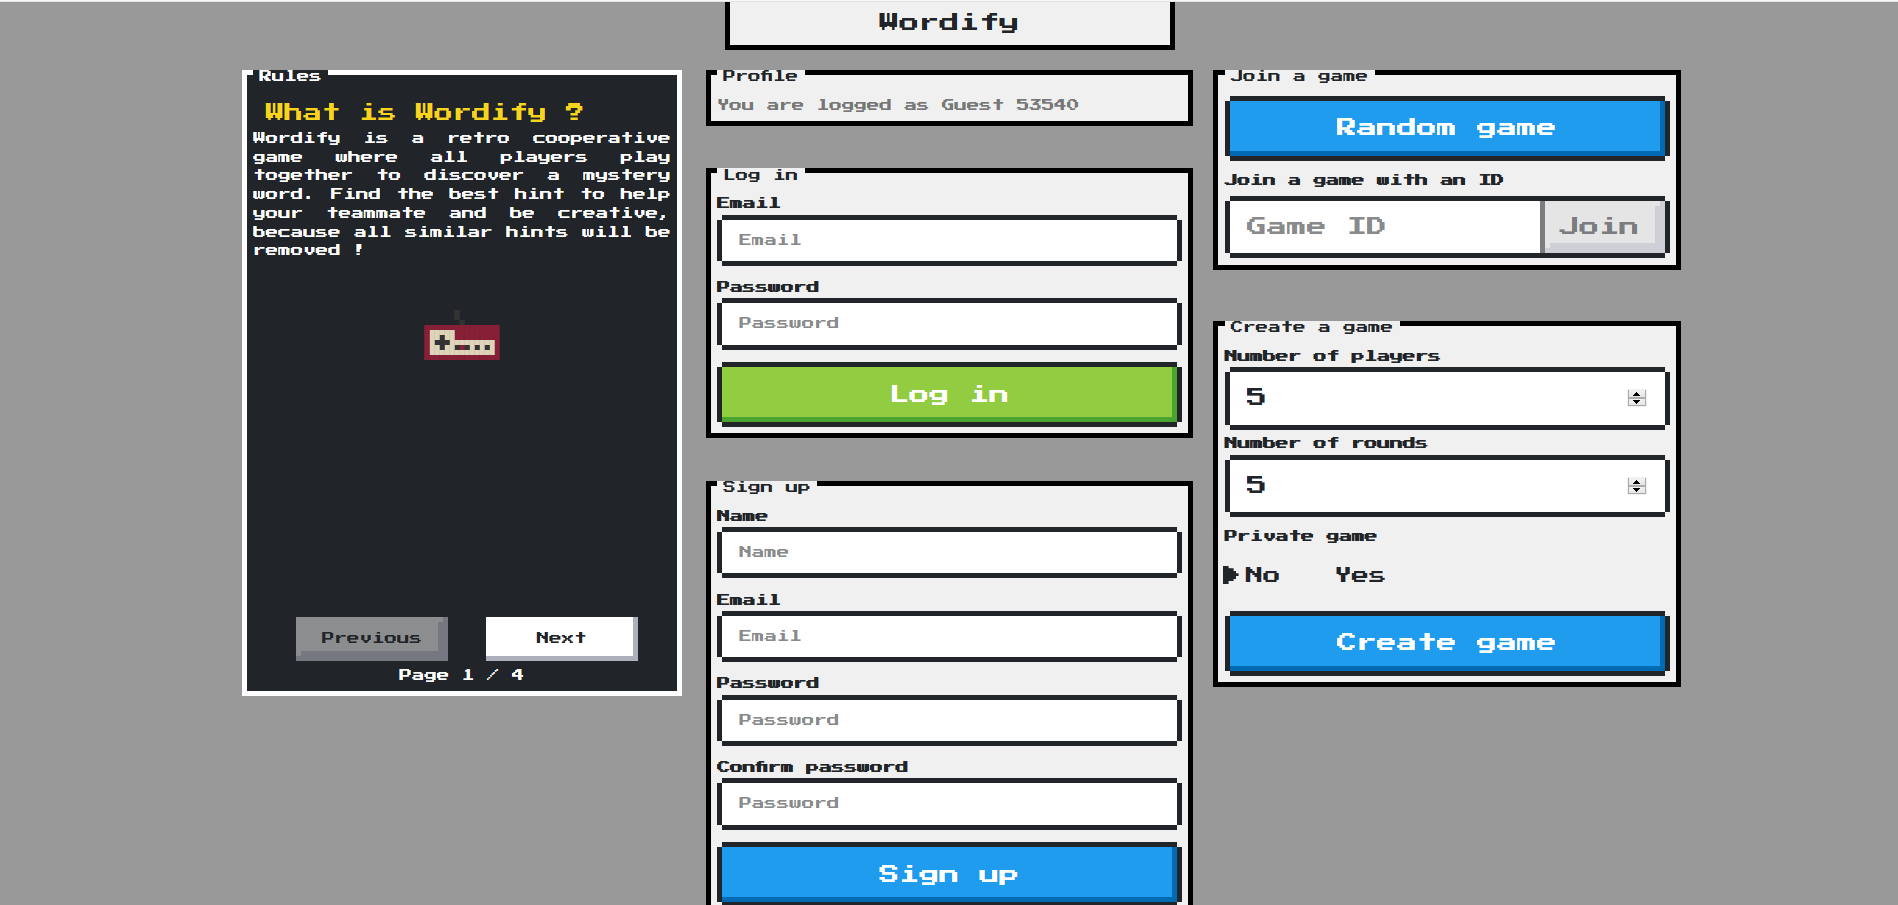
\includegraphics[scale=0.24]{figures/wordify_home_page}
	\label{fig:wordify_home_page}
	\caption{Wordify home page}
\end{figure} 

\clearpage

\section{Rules}

Once the players are connected to a game, the first round will automatically be initialized with the designation of an active player. An active player is the player who will have to guess the word according to the indices proposed by his teammates. Once the player selection is made, the system selects a word among a list stored in the database. This action completes the initialization phase for the first round. 

The mystery word is then displayed to non-active players. Then, they have to write a word related to the word to be divined by the active player, by respecting the time limit. In parallel, they must be careful not to put obvious words that other players could write. For the game to be interesting, it is important that players do not agree on the word they choose. If if it is the case, the interest of the game is lost. 

When the words have been entered by the other players, they are displayed to the active player so that he can guess the initial word. Be careful, identical or similar words will be removed from the list of words displayed to the active player. That is why it is wise to find words from the semantic field referring to the word to be guessed. 

In the next round, a new player is designated as active. The same rules are applied for this new round. The game ends when the number of rounds, indicated at the game creation, have been completed. The goal is to get the maximum number of points, knowing that, in case of bad answer from the active player, the team looses 2 points and in case of non-proposal, it will lose 1 point. 

A player can play games as many times as he wants. He can re-share the link of his new game to invite people ha wants to play with. This game is fun and challenging !

\section{Educational aspect}

In order to foster English education, this game has an educational purpose. Indeed, its goal is to learn new words from other players and to expand our vocabulary. Moreover, it combines speed and reflection : this is therefore and effective way to reason quickly in English while having a good time. In this way, this game targets anyone wishing to improve their level English level while avoiding long courses. it makes accessible the practice of English by providing a ludic way to learn it. 

In addition, such a game enables teachers to create contexts where English language is useful and meaningful. Even though games are often associated with entertainment, we do not have to forget their educational value, especially in teaching and learning foreign languages. Games are effective in the way that they create motivation, reduce student stress and enable language learners to communicate.

\cleardoublepage

\chapter{User documentation}

\section{Interface}

\section{Functionalities}

\subsection{Game creation}

\subsection{Guess a word}

\subsection{Enter a word}

\subsection{...}

\section{Other functionalities}

\cleardoublepage

\chapter{Documentation technique}

Dans cette quatrième partie, on souhaite présenter la mise en oeuvre informatique suivie quant à notre jeu en ligne. Pour cela, on a décidé de diviser ce chapitre selon les technologies utilisées pour la partie non-visible par l'utilisateur (Back-End), la partie visible (Front-End) et la stratégie de déploiement adoptée pour que la solution soit accessible en ligne. Ces trois sous-parties sont ensuite compétées par la présentation de problèmes rencontrés et les solutions trouvées pour les résoudre. 

\section{Back-end}

\subsection{Laravel}

On souhaite donc débuter par la description de la partie serveur, qui correspond donc à l'ensemble non-visible par l'utilisateur. Ainsi, pour structurer notre projet de la manière la plus efficace qui soit, nous avons fait le choix d'utiliser le framework Laravel qui permet de suivre le patron de conception appelé \textit{Modèle-Vue-Contrôleur} (MVC). En utilisant cet outil actuellement très employé pour la création d'applications Web, nous avons pu utiliser des fonctionnalités déjà présentes nous permettant de nous concentrer principalement sur le développement de la solution en tant que telle.

// Langage PHP

\subsection{Sockets}

Pour éviter des rechargements inopinés de la page de jeu, nous avons fait en sorte d'utiliser des sockets. Cette technologie permet de communiquer avec le serveur sans avoir à recharger la page sur laquelle on se trouve pour voir des potentiels changements s'afficher. Ceci garantit donc une navigation plus agréable à l'utilisateur final lorsque celui effectue des actions dont le serveur est à l'écoute. 

Nous avons donc dû utiliser des outils complémentaires et veiller à les associer au sein du framework Laravel. Cette phase a constitué une partie importante de notre travail. En effet, nous avons dû utiliser un outil supplémentaire côté serveur. Cet outil est appelé \textit{Redis}. Il permet de sauvegarder les événements déclenchés par le serveur en réaction aux interactions faites par un ou plusieurs joueurs.

\subsection{API externe}

\section{Front-End}

\subsection{Langages de programmation}

\subsection{Design}

// NES CSS \\
// COULEURS UTILISEES

\subsection{Sockets}

// EVITER REFRESH DE PAGE

\section{Déploiement}

// DOCKER \\
// DEPLOIEMENT SUR SERVEUR (ACCESSIBLE EN LIGNE) \\
// NOM DE DOMAINE \\

\section{Architecture globale}
!
// COMMENT TOUT COMMUNIQUE ? => DIAGRAMME D'ARCHITECTURE SYNTHETIQUE

\section{Problèmes rencontrés}

\subsection{Solutions adoptées}

\cleardoublepage

\chapter{Scénario}

\cleardoublepage

\appendix
\part*{Annexes}
\addcontentsline{toc}{part}{Annexes}

// METTRE DES SCREENSHOTS DES DIFFERENTES INTERFACES \\
// METTRE UN EXEMPLE DE JSON UTILISE POUR UNE PARTIE \\
// LIENS VERS LES TECHNOS UTILISEES

\end{document}
